\documentclass{ieeeojies}
\usepackage{cite}
\usepackage{amsmath,amssymb,amsfonts}
\usepackage{algorithmic}
\usepackage{graphicx}
\usepackage{textcomp}
\usepackage{array}
\usepackage[table]{xcolor}
\usepackage{multirow}
\usepackage{multicol}
\usepackage{float}

\def\BibTeX{{\rm B\kern-.05em{\sc i\kern-.025em b}\kern-.08em
    T\kern-.1667em\lower.7ex\hbox{E}\kern-.125emX}}

\begin{document}
\title{\Large{Harnessing Advanced Algorithms for Cryptocurrency Price Prediction}}
\vspace{-10mm}
\author{{Bui Van Thai}\authorrefmark{1},
  {Nguyen Binh Nguyen\authorrefmark{2}, and Nguyen The Vinh}\authorrefmark{3}}
\address[1]{21522577, Faculty of Information Systems, University of Information Technology, (e-mail: 21522577@gm.uit.edu.vn)}
\address[2]{21522391, Faculty of Information Systems, University of Information Technology, (e-mail: 21522391@gm.uit.edu.vn)}
\address[3]{21522794, Faculty of Information Systems, University of Information Technology, (e-mail: 21522794@gm.uit.edu.vn)}
\markboth
{Author \headeretal: Bui Van Thai, Nguyen Binh Nguyen, Nguyen The Vinh}
{Author \headeretal: Bui Van Thai, Nguyen Binh Nguyen, Nguyen The Vinh}
% \vspace{-10mm}
\begin{abstract} \par
  Unlocking the potential of accurate Bitcoin price predictions, this study introduces eight powerful algorithms - SES, GARCH, MLP,
  Linear Regression, ARIMA, RNN, GRU, and LSTM - that harness the strengths of exponential smoothing, volatility modeling, regression
  analysis, time series forecasting, and various neural network architectures to forecast the future price movements of the cryptocurrency.
  These algorithms were chosen due to their respective strengths in capturing short-term trends (SES), volatility dynamics (GARCH),
  linear relationships (Linear Regression), autoregressive patterns (ARIMA), and complex nonlinear patterns (MLP, RNN, GRU, LSTM).
  By combining these algorithms, we aim to provide a comprehensive and accurate framework for forecasting Bitcoin prices, offering valuable
  insights for investors in the cryptocurrency market.\\
  \\
  \textbf{Keywords:} Bitcoin price prediction, cryptocurrency forecasting, SES, GARCH, Linear Regression, ARIMA, RNN, GRU, LSTM, MLP, time series analysis, neural networks, financial modeling.
\end{abstract}
\titlepgskip=-40pt
\maketitle
\section{Introduction}
The prediction of cryptocurrency prices has garnered significant attention in recent years due to the increasing popularity and market
impact of digital currencies. Among the various cryptocurrencies, Bitcoin stands out as the most prominent and widely traded one.
The ability to accurately forecast Bitcoin prices has the potential to provide valuable insights for investors, traders, and policymakers
in understanding the dynamics of this volatile market.

\noindent In this study, we apply eight forecasting algorithms, namely Generalized Autoregressive Conditional Heteroskedasticity (GARCH),
Single Exponential Smoothing (SES), Multilayer Perceptron (MLP), Linear Regression, AutoRegressive Integrated Moving Average (ARIMA),
Recurrent Neural Networks (RNN), Gated Recurrent Unit (GRU), and Long Short-Term Memory (LSTM), to predict the price of Bitcoin.
These algorithms have been widely used in financial forecasting and have demonstrated effectiveness in capturing
the time-varying characteristics and nonlinear patterns present in financial data.

\noindent The GARCH model, proposed by Bollerslev (1986) \cite{b1}, is a popular choice for modeling the volatility of financial time series. It takes into
account the conditional heteroskedasticity, allowing for the estimation of time-varying volatility. The SES method, introduced by Brown (1956) \cite{b2},
is a simple and widely used exponential smoothing technique that assigns exponentially decreasing weights to past observations. The MLP algorithm, a type of
artificial neural network, has gained attention for its ability to capture complex relationships and nonlinearity in data \cite{b7}. Linear Regression is
a fundamental statistical method used to model the relationship between a dependent variable and one or more independent variables \cite{b10}. ARIMA,
introduced by Box and Jenkins \cite{b8}, is a widely used statistical method for time series forecasting that combines autoregression, differencing,
and moving averages. RNN, GRU, and LSTM are advanced neural network architectures specifically designed to handle sequential data and
capture long-term dependencies \cite{b9}.

\noindent To evaluate the performance of these forecasting algorithms, we utilize a comprehensive dataset of Bitcoin prices spanning multiple years.
The dataset includes historical price data, as well as other relevant features such as trading volume, market capitalization, and sentiment analysis indicators.
By incorporating these additional factors, we aim to enhance the predictive accuracy of the models and provide a more comprehensive analysis of Bitcoin price movements.

\noindent The primary objectives of this study are twofold. First, we aim to compare the forecasting performance of the GARCH, SES, MLP, Linear Regression,
ARIMA, RNN, GRU, and LSTM algorithms in predicting Bitcoin prices. By assessing the accuracy and robustness of these models, we can gain insights into
their suitability for cryptocurrency price prediction. Second, we seek to identify the key factors that contribute to the prediction accuracy, shedding light
on the underlying drivers of Bitcoin price dynamics.

\label{sec:introduction}

\section{Related Works}
In recent years, there has been a substantial amount of research dedicated to predicting stock prices using various machine learning and statistical models. \\
Linear Regression is a fundamental and widely used statistical technique in financial forecasting due to its simplicity and interpretability. Kumar and Thenmozhi (2006) \cite{b10} applied this model to predict stock prices of major Indian companies, demonstrating its ability to capture market trends. However, Patel et al. (2015) showed that more complex models like SVM and ANN often outperform Linear Regression in predicting stock prices, especially in capturing complex patterns.\\
RNNs (Recurrent Neural Networks) are specialized neural networks designed for sequential data processing, particularly suitable for time series forecasting. Zhang et al. (2019) \cite{b11} employed RNNs to forecast Bitcoin prices, showcasing their ability to capture complex and nonlinear time series patterns .\\
GRU (Gated Recurrent Unit) networks, similar to LSTMs but with a simpler architecture, have been applied to forecast stock prices effectively. Chung et al. (2014) \cite{b12} empirically evaluated GRUs and found them comparable to LSTMs in forecasting tasks while requiring fewer computational resources.\\
ARIMA (The AutoRegressive Integrated Moving Average) model is a powerful statistical technique widely used for time series forecasting. Tsai et al. (2010) \cite{b13} utilized ARIMA to forecast stock prices and stock market indices, highlighting its effectiveness in capturing linear time series patterns .\\
GARCH models have been used to catch the price volatility of different commodities and assets. It was proved that GARCH model is a suitable approach to detect the volatility along the meat supply chain \cite{b3}. The GARCH model has also been used for forecasting the volatility of the Islamic stock index \cite{b4}, Bitcoin \cite{b14}, and bond yield \cite{b6}.\\
SES (Single Exponential Smoothing) is a simple yet effective time series forecasting method. Ostertagova, Eva \& Ostertag, Oskar \cite{b30} utilized SES to predict primary production of electricity Slovakia for the year 2010. Their results showed that SES performed well in capturing the trend and short-term fluctuations.\\
Long Short-Term Memory (LSTM) networks, a type of RNN, are designed to address the vanishing gradient problem and capture long-term dependencies. Fischer and Krauss (2018) \cite{b15} highlighted LSTM's superiority over traditional models and other machine learning algorithms in predicting stock prices, due to its ability to model both short-term fluctuations and long-term trends.\\
MLP (Multilayer Perceptron) is a type of artificial neural network that has been widely used in financial forecasting tasks. Zhang et al. (2019) \cite{b7} employed MLP models to predict Bitcoin prices and evaluated their performance against other machine learning algorithms. The results demonstrated that MLP models achieved high accuracy in forecasting Bitcoin prices, especially in capturing complex patterns and nonlinear relationships.

\section{Materials}
\subsection{Dataset}
Historical price data for Binance Coin (BNB), Dogecoin, and Tron from 01/03/2019 to 01/06/2024 will be applied. The data contains column such as Date, Price, Open, High, Low, Vol., Change. As the goal is to forecast close prices, only data relating to column “Price" (USD) will be processed.

\subsection{Descriptive Statistics}
\begin{table}[H]
  \centering
  \caption{BNB, DOGECOIN, TRON's Descriptive Statistics}
  \begin{tabular}{|>{\columncolor{yellow!20}}c|c|c|c|}
    \hline
    \rowcolor{yellow!20} & BNB       & DOGECOIN & TRON     \\ \hline
    Count                & 1920      & 1920     & 1920     \\ \hline
    Mean                 & 229.552   & 0.083    & 0.059    \\ \hline
    Var                  & 33996.748 & 0.009    & 0.001    \\ \hline
    Std                  & 184.382   & 0.093    & 0.034    \\ \hline
    Min                  & 9.25      & 0.001585 & 0.008409 \\ \hline
    25\%                 & 27.03     & 0.0029   & 0.025    \\ \hline
    50\%                 & 247.55    & 0.0672   & 0.062    \\ \hline
    75\%                 & 332.11    & 0.119    & 0.080    \\ \hline
    Max                  & 676.56    & 0.68688  & 0.1639   \\ \hline
  \end{tabular}
\end{table}

\begin{figure}[H]
  \centering
  \begin{minipage}{0.23\textwidth}
    \centering
    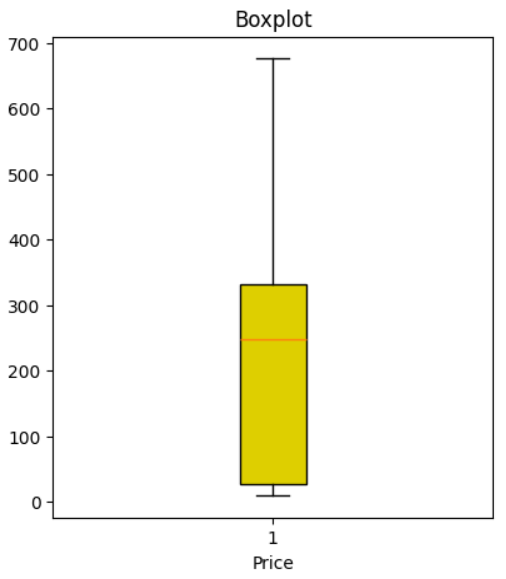
\includegraphics[width=1\textwidth]{Image/Discriptive/boxplot_bnb_new.png}
    \caption{BNB coin price's boxplot}
    \label{fig:1}
  \end{minipage}
  \hfill
  \begin{minipage}{0.23\textwidth}
    \centering
    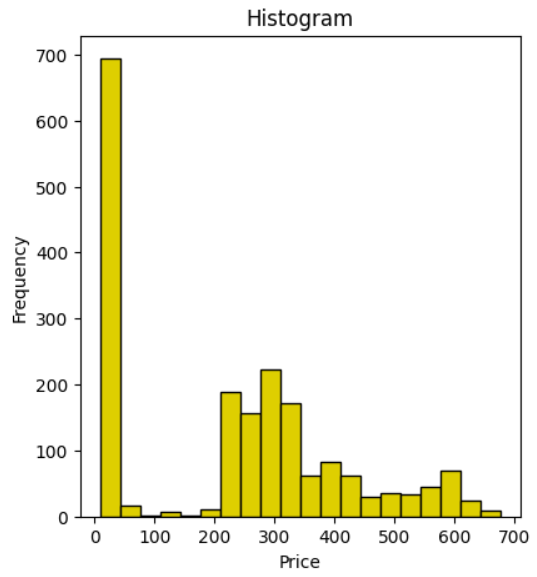
\includegraphics[width=1\textwidth]{Image/Discriptive/histo_bnb_new.png}
    \caption{BNB coin price's histogram}
    \label{fig:2}
  \end{minipage}
\end{figure}

\begin{figure}[H]
  \centering
  \begin{minipage}{0.23\textwidth}
    \centering
    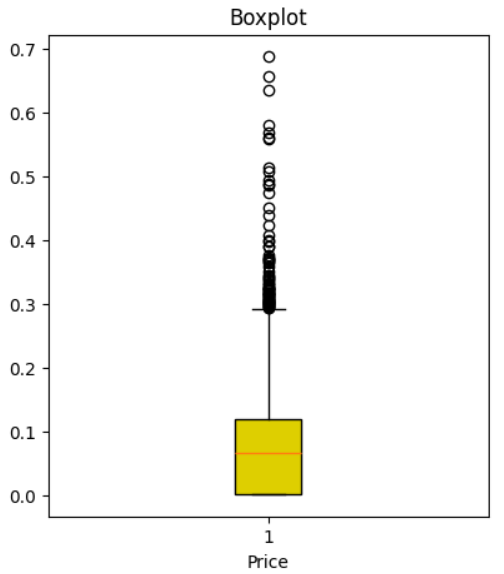
\includegraphics[width=1\textwidth]{Image/Discriptive/boxplot_doge_new.png}
    \caption{Dogecoin coin price's boxplot}
    \label{fig:3}
  \end{minipage}
  \hfill
  \begin{minipage}{0.23\textwidth}
    \centering
    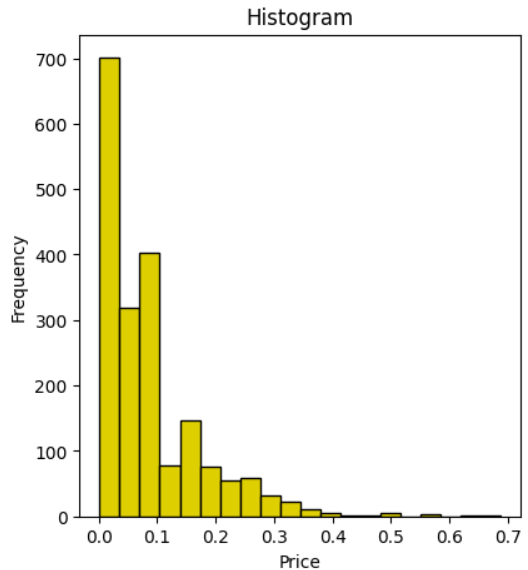
\includegraphics[width=1\textwidth]{Image/Discriptive/histo_doge_new.png}
    \caption{Dogecoin coin price's histogram}
    \label{fig:4}
  \end{minipage}
\end{figure}

\begin{figure}[H]
  \centering
  \begin{minipage}{0.23\textwidth}
    \centering
    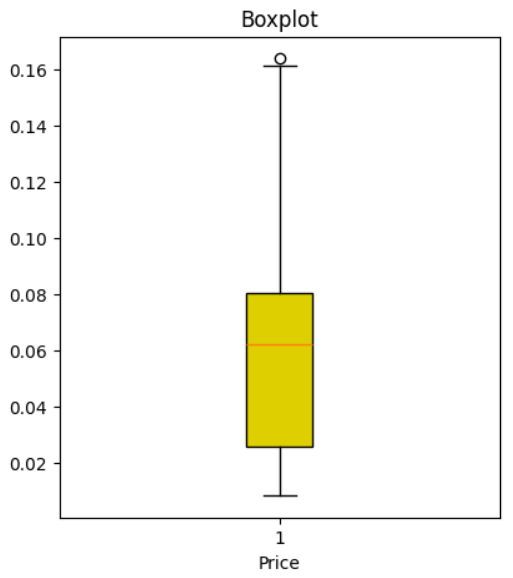
\includegraphics[width=1\textwidth]{Image/Discriptive/boxplot_tron_new.png}
    \caption{Tron coin price's boxplot}
    \label{fig:5}
  \end{minipage}
  \hfill
  \begin{minipage}{0.23\textwidth}
    \centering
    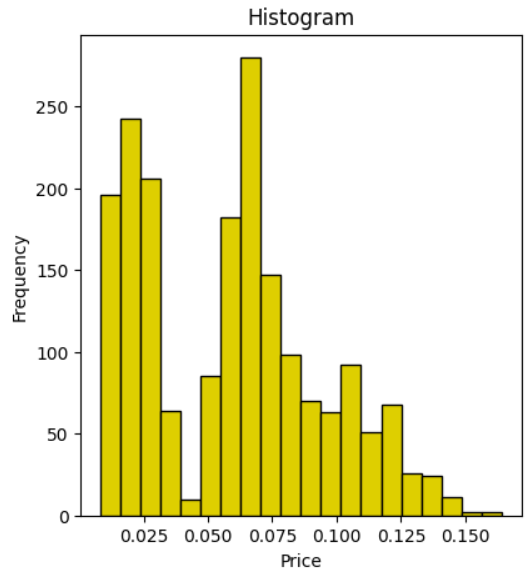
\includegraphics[width=1\textwidth]{Image/Discriptive/histo_tron_new.png}
    \caption{Tron coin price's histogram}
    \label{fig:6}
  \end{minipage}
\end{figure}

\section{Methodology}

\subsection{GARCH}
The GARCH (Generalized Autoregressive Conditional Heteroskedasticity) model is a crucial tool in finance for forecasting
the volatility of time series. This model allows for time-varying volatility, providing
a more accurate description of fluctuations in financial data. The formula of the GARCH(p,q) model is:
\[
  \sigma^2_t = \omega + \sum_{i=1}^{p} \alpha_i \varepsilon^2_{t-i} + \sum_{j=1}^{q} \beta_j \sigma^2_{t-j}
\]

Where:
\begin{itemize}
  \item \(\sigma^2_t\) represents the conditional variance at time \(t\).
  \item \(\omega\) is the constant term or intercept.
  \item \(\alpha_i\) (\(i=1, \ldots, p\)) are the coefficients associated with the past squared error terms (ARCH terms).
  \item \(\beta_j\) (\(j=1, \ldots, q\)) are the coefficients associated with the past conditional variances (GARCH terms).
  \item \(\varepsilon^2_{t-i}\) are the past error terms, calculated as:
        \[
          \varepsilon_{t-i} = y_{t-i} - \mu
        \]
        where \(y_{t-i}\) is the observed value at time \(t-i\) and \(\mu\) is the mean of the time series.
  \item \(\sigma^2_{t-j}\) are the past conditional variances, calculated recursively using the GARCH model.
\end{itemize}

In order for \(\sigma^2_t > 0\), it is assumed that \(\omega > 0\) and the coefficients \(\alpha_i\) (\(i=1, \ldots, p\)) and \(\beta_j\) (\(j=1, \ldots, q\)) are all non-negative.
When \(q=0\), the GARCH(p,q) model reduces to the ARCH(p) model.

Usually, the GARCH(1,1) model,
\[
  \sigma^2_t = \omega + \alpha_1 \varepsilon^2_{t-1} + \beta_1 \sigma^2_{t-1},
\]
with only three parameters in the conditional variance equation, is adequate to obtain a good model fit for daily asset returns. Indeed, Hansen and Lund (2004) provided compelling evidence that it is difficult to find a volatility model that outperforms the simple GARCH(1,1). Hence, for many purposes, the GARCH(1,1) model is the de facto volatility model of choice for daily returns \cite{b1}.

Given its effectiveness in modeling daily asset returns, the GARCH(1,1) model is also suitable for forecasting the volatility of cryptocurrencies such as Bitcoin. Cryptocurrencies often exhibit high volatility, and the GARCH(1,1) model's ability to adapt to changing volatility over time makes it a practical choice for this application.

\subsection{Recurrent Neural Networks (RNNs)}
Recurrent Neural Networks (RNNs) are a class of artificial neural networks designed for sequence modeling, commonly used in tasks such as time series prediction, natural language processing, and speech recognition. Unlike traditional feedforward neural networks, RNNs have connections that form directed cycles, allowing them to maintain a form of memory of previous inputs through their internal state. The general form of an RNN can be described by the following equations:

\[
  h_t = \sigma_h(W_h x_t + U_h h_{t-1} + b_h)
\]

\[
  y_t = \sigma_y(W_y h_t + b_y)
\]

Where:
\begin{itemize}
  \item \( h_t \) represents the hidden state at time \( t \).
  \item \( x_t \) is the input at time \( t \).
  \item \( y_t \) is the output at time \( t \).
  \item \( W_h \) is the weight matrix for the input to hidden state.
  \item \( U_h \) is the weight matrix for the hidden state to hidden state (recurrent connection).
  \item \( W_y \) is the weight matrix for the hidden state to output.
  \item \( b_h \) and \( b_y \) are the bias vectors for the hidden state and output, respectively.
  \item \( \sigma_h \) and \( \sigma_y \) are the activation functions for the hidden state and output, respectively.
  \item \( h_{t-1} \) is the hidden state at the previous time step \( t-1 \).
\end{itemize} \cite{b16,b18,b19}

\subsection{ARIMA}
ARIMA (Autoregressive Integrated Moving Average) is a time series forecasting model that combines autoregression (AR), differencing (I), and moving average (MA) components. It is commonly used to predict future values based on past observations.
\begin{itemize}
  \item AR (Autoregressive): Autocorrelation property of the data with itself at previous time points. The ARIMA model uses parameter \(\rho\) to determine the number of previous values to compute.
  \item I (Integrated): The integration step is to make the data easily predictable by removing trends in the data. This is often done by taking the difference between consecutive data points. The ARIMA model uses parameter \(\Bar{d}\) to determine the number of differencing steps.
  \item MA (Moving Average): Used to model random fluctuations in the data. The ARIMA model uses parameter \(\Bar{q}\) to determine the number of moving average values \cite{b8, b9, b13}.
\end{itemize}

\subsection{Gated Recurrent Unit(GRU)}
GRU is a type of recurrent neural network (RNN) designed to handle and predict sequence data, such as time series data. GRU was first introduced by K. Cho et al. in 2014 as an improvement over Long Short-Term Memory (LSTM), another RNN model, with the aim of simplifying the architecture and reducing the number of parameters. GRU consists of two main gates:
\begin{itemize}
  \item Update Gate: Determines how much of the previous state needs to be retained.
  \item Reset Gate: Determines how much of the previous state needs to be forgotten.
\end{itemize}
The computational formulas for GRU are:
\begin{itemize}
  \item Update Gates: \[z_t = \sigma(W_z \cdot [h_{t-1}, x_t]) \]
  \item Reset Gate: \[r_t = \sigma(W_r \cdot [h_{t-1}, x_t])\]
  \item Candidate State: \[\tilde{h} = \tanh(W \cdot [r_t*h_{t-1}, x_t])\]
  \item New State: \[h_t = (1 - z_t) * h_{t-1} + z_t * \tilde{h}_t \]
\end{itemize}
Where:
\begin{itemize}
  \item \(x_t\): is the input at time t.
  \item \(h_t\): is the hidden state at time t.
  \item \(W_z, W_r, W\): are weight matrices.
  \item \(\sigma\): is the sigmoid function.\cite{b12, b20, b21}
\end{itemize}
\begin{figure}[H]
  \centering
  \begin{minipage}{1\linewidth}
    \centering
    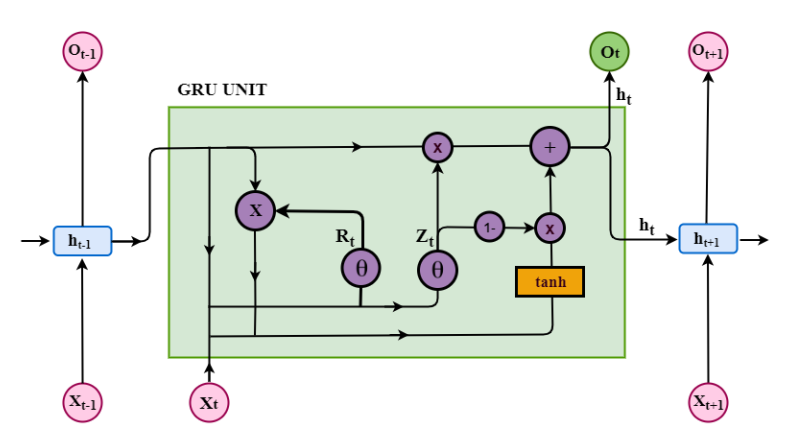
\includegraphics[width=\linewidth]{Image/GRU/model_gru.png}
    \caption{The Architecture of basic Gated Recurrent Unit (GRU).}
    \label{fig:7}
  \end{minipage}
\end{figure}
\subsection{Multilayer Perceptron(MLP)}
MLP is a type of neural network with a simple structure and forms the basis of many other neural network architectures. An MLP consists of at least three layers: an input layer, one or more hidden layers, and an output layer. Each layer in an MLP is a set of perceptrons, and each perceptron is a computational unit that performs matrix multiplication and applies an activation function.The structure of a typical MLP includes:
\begin{itemize}
  \item Input Layer: Receives input data.
  \item Hidden Layer(s): Processes and extracts features from the input data through weights and activation functions.
  \item Output Layer: Produces the final prediction result.
\end{itemize}
Each perceptron in a layer operates according to the formula:
\[y = \phi(W \cdot x + b)\]
Where:
\begin{itemize}
  \item x is the input.
  \item W is the weight vector.
  \item b is the bias.
  \item \(\phi\) is the activation function (commonly sigmoid, tanh, or ReLU).\cite{b16, b22, b23}
\end{itemize}
\begin{figure}[H]
  \centering
  \begin{minipage}{0.8\linewidth}
    \centering
    \includegraphics[width=\linewidth]{Image/MLP/model.png}
    \caption{A basic MLP model framework.}
    \label{fig:7}
  \end{minipage}
\end{figure}
\subsection{Linear Regression(LR)}
Regression analysis is a tool for building mathematical and statistical models that characterize relationships between a dependent variable and one or more independent, or explanatory, variables, all of which are numerical. This statistical technique is used to find an equation that best predicts the y variable as a linear function of the x variables.
A multiple linear regression model has the form:
\[Y=\beta_0+\beta_1X_1+\beta_2X_2+\cdots+\beta_kX_k+\varepsilon\]
Where:\\
\indent\textbullet\ Y is the dependent variable (Target Variable).\\
\indent\textbullet\ \(X_1, X_2, \ldots, X_k\) are the independent (explanatory) variables.\\
\indent\textbullet\ \(\beta_0\) is the intercept term.\\
\indent\textbullet\ \(\beta_1,..., \beta_k\) are the regression coefficients for the independent variables.\\
\indent\textbullet\ \(\varepsilon\) is the error term. \cite{b38, b39}

\subsection{Simple Exponential Smoothing(SES)}
Exponential smoothing is a forecasting method for univariate time series data. This method produces forecasts that are weighted averages of past observations where the weights of older observations exponentially decrease. The simplest of the exponentially smoothing methods is naturally called simple exponential smoothing (SES). Use simple exponential smoothing for univariate time series data that do not have a trend or seasonal cycle.
Forecasts are calculated using weighted averages, where the weights decrease exponentially as observations come from further in the past — the smallest weights are associated with the oldest observations:
\[
  \hat{y}_{t+1|t} = \alpha y_t + (1 - \alpha) \hat{y}_{t|t-1}
\]
Where:
\begin{itemize}
  \item \(\hat{y}_{t+1|t}\) the forecasted value at time based on \({t+1}\) information up to time \({t}\).
  \item \(\hat{y}\) the observed value at time \({t}\).
  \item \(\hat{y}_{t|t-1}\) the forecasted value at time \({t}\) based on information up to time \({t-1}\).
  \item \(\alpha\) the smoothing factor, which is a value between 0 and 1 that determines the influence of the current observation on the forecast. \cite{b26,b27}
\end{itemize}
\subsection{Long Short-Term Memory(LSTM)}
LSTM (Long Short-Term Memory) is a specialized type of Recurrent Neural Network (RNN) designed to handle long-term dependencies in sequential data. LSTM units consist of a cell state and three gates (input, forget, and output) that regulate the flow of information. The cell state maintains long-term information, while the gates control what information is added, retained, or output at each time step. This structure allows LSTMs to effectively mitigate the vanishing gradient problem common in traditional RNNs, making them well-suited for applications like speech recognition, time series prediction, and natural language processing. A basic LSTM unit consists of the following main components:
\begin{itemize}
  \item Cell State: Carries information across time steps, the cell state has the ability to maintain and regulate information over long periods.
  \item Forget Gate: Decides what information from the previous cell state should be forgotten.
  \item Input Gate: Decides what new information will be added to the cell state.
  \item Output Gate: Determines which part of the current cell state will be output.
  \item Cell State Update: Combines old and new information to update the cell state.
\end{itemize}
The computational formulas for LSTM are:
\begin{itemize}
  \item Forget Gate: \[f_t = \sigma(W_f \cdot [h_{t-1}, x_t] + b_f)\]
  \item Input Gate: \[i_t = \sigma(W_i \cdot [h_{t-1}, x_t] + b_i)\]
        \[\tilde{C}_t = \tanh(W_C \cdot [h_{t-1}, x_t] + b_C)\]
  \item Output Gate: \[o_t = \sigma(W_o \cdot [h_{t-1}, x_t] + b_o)\]
        \[h_t = o_t \cdot \tanh(C_t)\]
  \item Cell Update: \[C_t = f_t \cdot C_{t-1} + i_t \cdot \tilde{C}_t\]
\end{itemize}
Where:
\begin{itemize}
  \item \( f_t \): Forget gate activation vector at time step \( t \)
  \item \( i_t \): Input gate activation vector at time step \( t \)
  \item \( o_t \): Output gate activation vector at time step \( t \)
  \item \( \tilde{C}_t \): Candidate cell state at time step \( t \)
  \item \( C_t \): Cell state vector at time step \( t \)
  \item \( h_t \): Hidden state vector at time step \( t \)
  \item \( x_t \): Input vector at time step \( t \)
  \item \( W_f, W_i, W_C, W_o \): Weight matrices for the forget, input, cell, and output gates, respectively
  \item \( b_f, b_i, b_C, b_o \): Bias vectors for the forget, input, cell, and output gates, respectively
  \item \( \sigma \): Sigmoid activation function
  \item \( \tanh \): Hyperbolic tangent activation function. \cite{b34, b35}
\end{itemize}
\begin{figure}[H]
  \centering
  \begin{minipage}{1.0\linewidth}
    \centering
    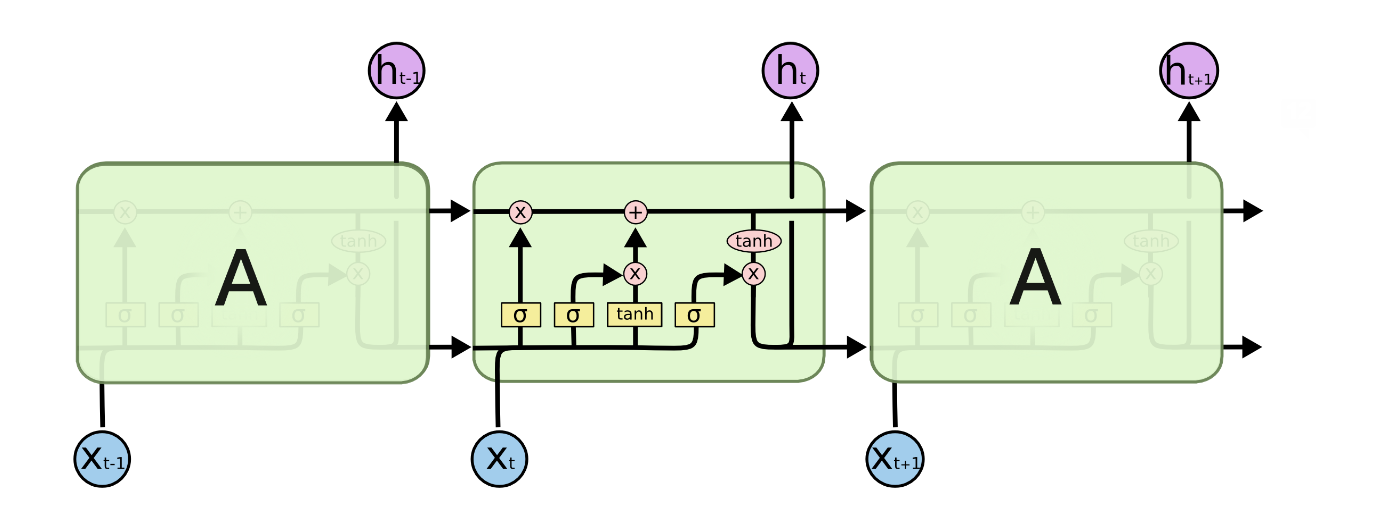
\includegraphics[width=\linewidth]{Image/LSTM/Model_LSTM.png}
    \caption{The repeating module in an LSTM.}
    \label{fig:8}
  \end{minipage}
\end{figure}
\section{Result}
\subsection{Evaluation Methods}
\textbf{Mean Percentage Absolute Error} (MAPE): is the average percentage error in a set of predicted values.

\[
  MAPE = \frac{100\%}{n} \sum_{i=1}^{n} \left| \frac{y_i - \hat{y_i}}{y_i} \right|
\]

Where: \\
\indent \textbullet\ \( n \) is the number of observations in the dataset. \\
\indent \textbullet\ \( y_i \) is the true value. \\
\indent \textbullet\ \( \hat{y_i} \) is the predicted value.

\textbf{Root Mean Squared Error} (RMSE): is the square root of the average value of the squared error in a set of predicted values.

\[
  RMSE = \sqrt{\frac{1}{n} \sum_{i=1}^{n} (\hat{y_i} - y_i)^2}
\]

Where: \\
\indent \textbullet\ \( n \) is the number of observations in the dataset. \\
\indent \textbullet\ \( y_i \) is the true value. \\
\indent \textbullet\ \( \hat{y_i} \) is the predicted value.
\textbf{Mean Absolute Error} (MSE):is a commonly used performance metric in machine learning and statistics. It measures the average of the squared differences
between the predicted values and the true/actual values.\\
\[
  MSE = \frac{1}{n} \sum_{i=1}^{n} \left( \log(1 + \hat{y_i}) - \log(\log(1 + y_i)) \right)^2
\]

Where: \\
\indent \textbullet\ \( n \) is the number of observations in the dataset. \\
\indent \textbullet\ \( y_i \) is the true value. \\
\indent \textbullet\ \( \hat{y_i} \) is the predicted value.
\vspace{-3mm}
\subsection{TRON Dataset}
\vspace{-2mm}
\begin{table}[H]
  \centering
  \begin{tabular}{|c|c|c|c|c|}
    \hline
    \multicolumn{5}{|c|}{\textbf{TRON Dataset's Evaluation}}                                     \\
    \hline
    \centering Model       & Training:Testing & RMSE           & MAPE (\%)      & MSE            \\
    \hline
    \multirow{2}{*}{LR}    & 7:3              & 0.0365         & 27.53          & 0.0013         \\ & \textbf{8:2} & \textbf{0.0365} & \textbf{27.53} & \textbf{0.0013} \\ & 9:1 & 0.0200 & 13.42 & 0.0004\\
    \hline
    \multirow{3}{*}{RNN}   & 7:3              & 0.003          & 2.82           & 6.96           \\ & 8:2 & 0.0024 & 1.8 & 5.59 \\ & \textbf{9:1} & \textbf{0.0026} & \textbf{1.74} & \textbf{6.87} \\
    \hline
    \multirow{2}{*}{GRU}   & 7:3              & 0.002          & 1.681          & 0.000004       \\ & 8:2 & 0.002 & 1.509 & 0.000004 \\ & \textbf{9:1} & \textbf{0.002}  & \textbf{1.355} & \textbf{0.000005}\\
    \hline
    \multirow{2}{*}{ARIMA} & 7:3              & 0.035          & 26.805         & 0.001          \\ & 8:2 &  0.036 & 27.547 & 0.001 \\ & \textbf{9:1} & \textbf{0.02}  & \textbf{13.423} &\textbf{0.0004}\\
    \hline
    \multirow{2}{*}{GARCH} & \textbf{7:3}     & \textbf{0.039} & \textbf{30.93} & \textbf{0.002} \\
                           & 8:2              & 0.063          & 57.03          & 0.004          \\
                           & 9:1              & 0.079          & 63.97          & 0.006          \\
    \hline
    \multirow{2}{*}{SES}   & 7:3              & 0.0365         & 27.53          & 0.0013         \\ & 8:2 & 0.0365 &27.53 & 0.0013\\ & \textbf{9:1} &  \textbf{0.0200} & \textbf{13.42} & \textbf{0.0004} \\
    \hline
    \multirow{2}{*}{LSTM}  & 7:3              & 0.0038         & 3.29           & 0.000014       \\ & \textbf{8:2} & \textbf{0.0029} & \textbf{2.00} &  \textbf{0.000008} \\ & 9:1 &  0.0034 &	2.30 & 0.000012 \\
    \hline
    \multirow{2}{*}{MLP}   & 7:3              & 0.002          & 0.017          & 0.000004       \\ & \textbf{8:2} & \textbf{0.002} & \textbf{0.014} &  \textbf{0.000004} \\ & 9:1 & 0.003 & 0.018 & 0.000007\\
    \hline
  \end{tabular}
  \caption{TRON Dataset's Evaluation}
  \label{tronresult}
\end{table}
\vspace{-10mm}
\begin{figure}[H]
  \centering
  \begin{minipage}{0.8\linewidth}
    \centering
    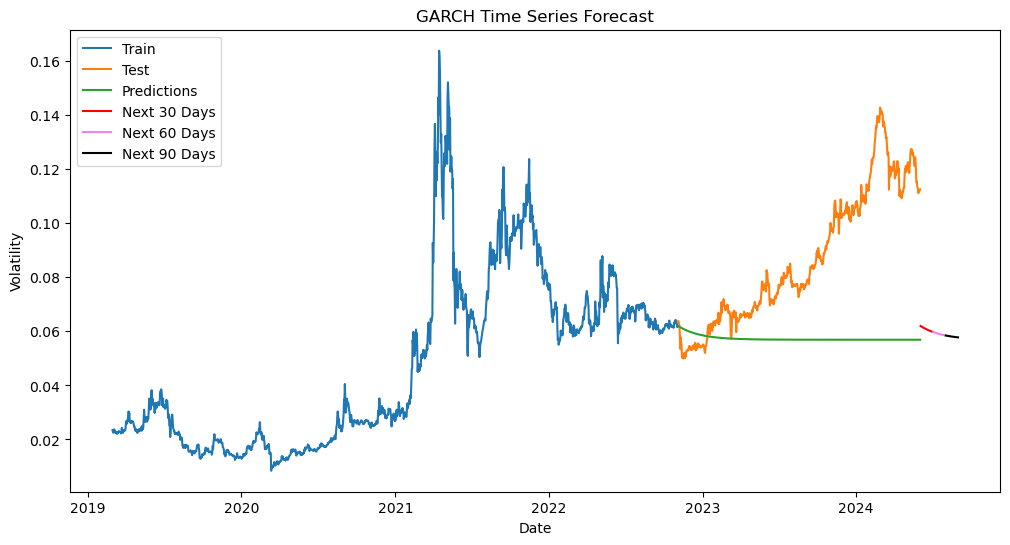
\includegraphics[width=\linewidth]{Image/Garch/GARCH_TRON73.png}
    \caption{GARCH model's result with 7:3 splitting proportion}
    \label{fig:7}
  \end{minipage}
\end{figure}
\vspace{-5mm}
\begin{figure}[H]
  \centering
  \begin{minipage}{0.8\linewidth}
    \centering
    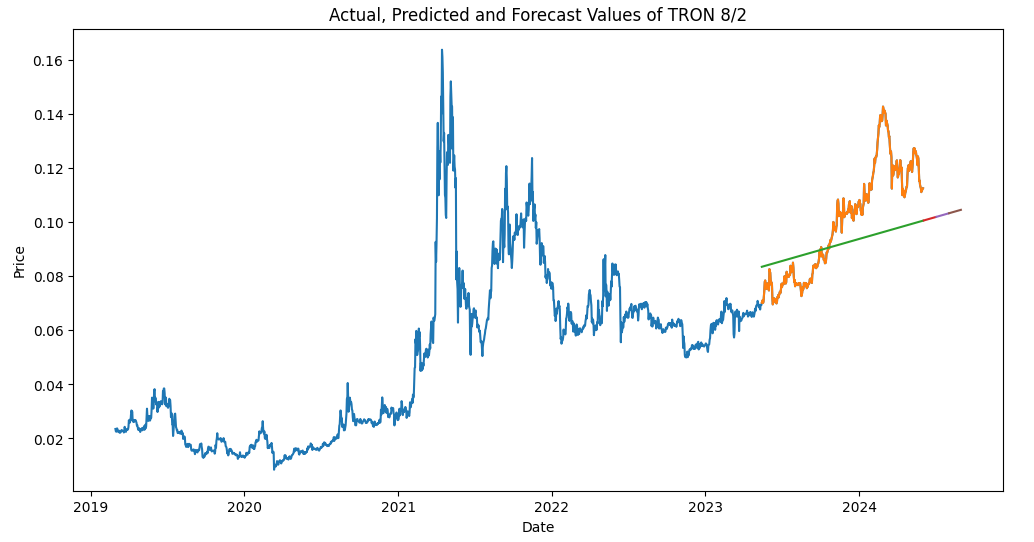
\includegraphics[width=\linewidth]{Image/LN/LN_TRON_82.png}
    \caption{LR model's result with 8:2 splitting proportion}
    \label{fig:8}
  \end{minipage}
\end{figure}
\vspace{-5mm}
\begin{figure}[H]
  \centering
  \begin{minipage}{0.8\linewidth}
    \centering
    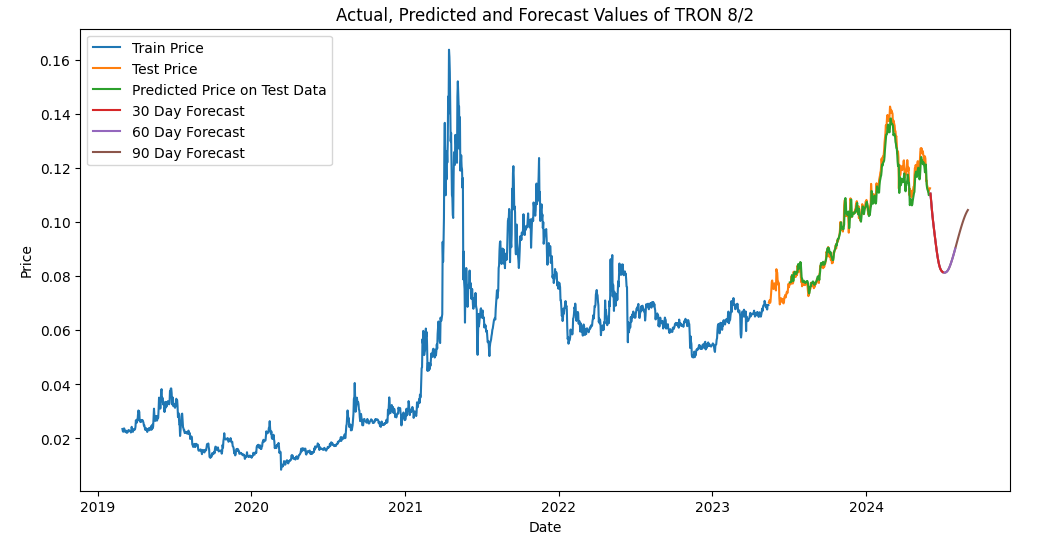
\includegraphics[width=\linewidth]{Image/LSTM/LSTM_TRON_82.png}
    \caption{LSTM model's result with 8:2 splitting proportion}
    \label{fig:9}
  \end{minipage}
\end{figure}
\vspace{-5mm}
\begin{figure}[H]
  \centering
  \begin{minipage}{0.8\linewidth}
    \centering
    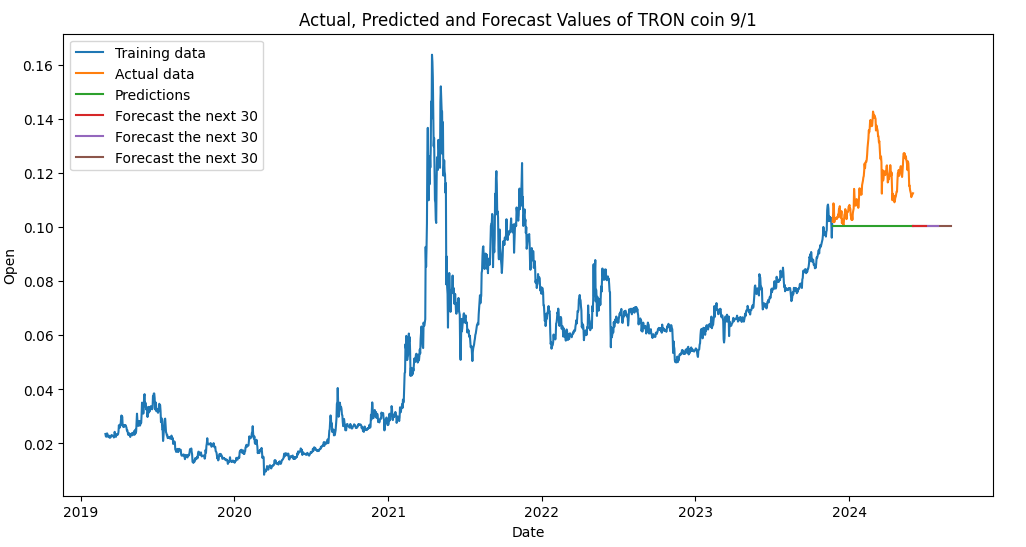
\includegraphics[width=\linewidth]{Image/SES/SES_TRON_91.png}
    \caption{SES model's result with 9:1 splitting proportion}
    \label{fig:10}
  \end{minipage}
\end{figure}
\vspace{-5mm}
\begin{figure}[H]
  \centering
  \begin{minipage}{0.8\linewidth}
    \centering
    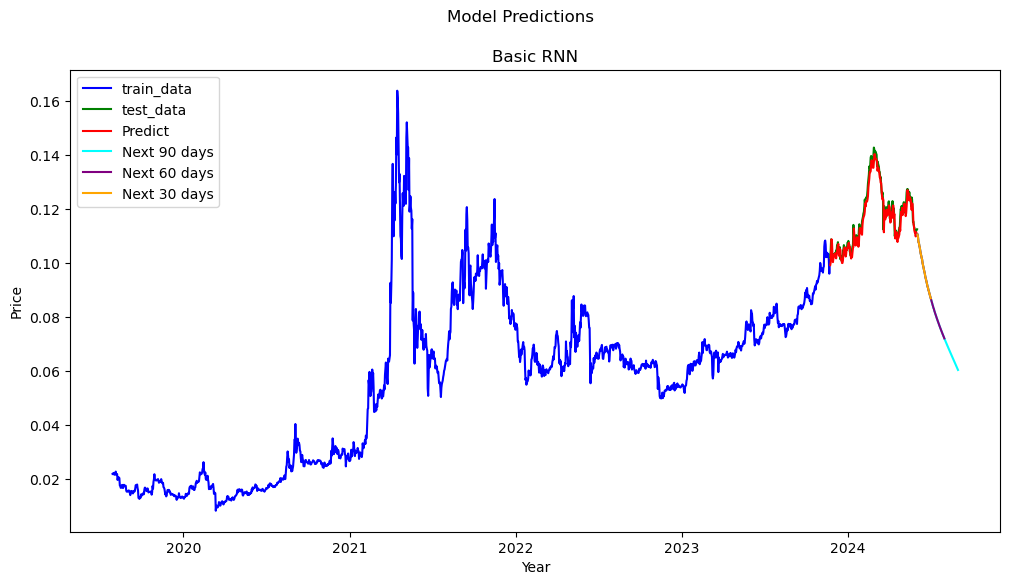
\includegraphics[width=\linewidth]{Image/RNN/RNN_TRON91.png}
    \caption{RNN model's result with 9:1 splitting proportion}
    \label{fig:11}
  \end{minipage}
\end{figure}
\vspace{-5mm}
\begin{figure}[H]
  \centering
  \begin{minipage}{0.8\linewidth}
    \centering
    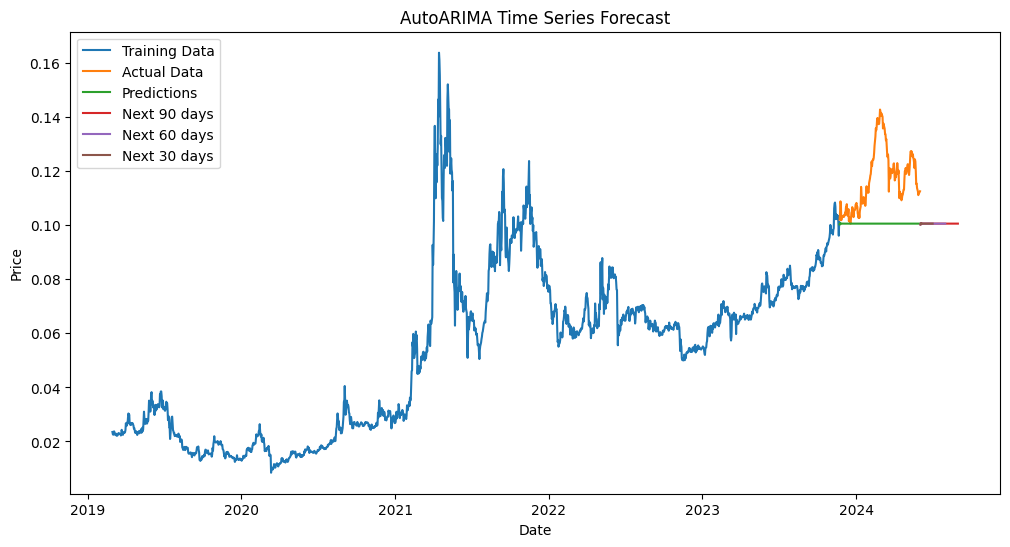
\includegraphics[width=\linewidth]{Image/Arima/Arima_tron_9_1_n.png}
    \caption{ARIMA model's result with 9:1 splitting proportion}
    \label{fig:12}
  \end{minipage}
\end{figure}
\vspace{-5mm}
\begin{figure}[H]
  \centering
  \begin{minipage}{0.8\linewidth}
    \centering
    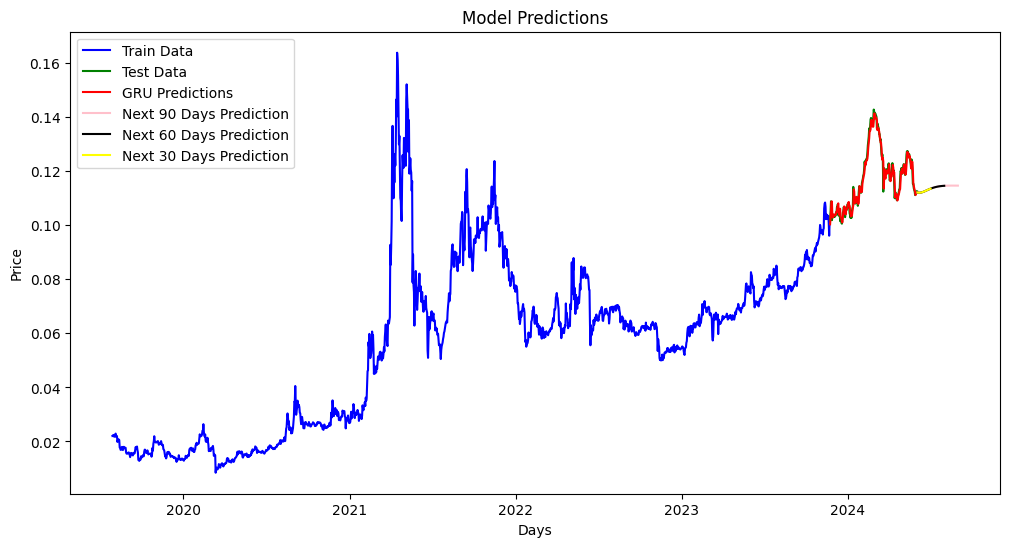
\includegraphics[width=\linewidth]{Image/GRU/GRU_TRON_91_n.png}
    \caption{GRU model's result with 9:1 splitting proportion}
    \label{fig:13}
  \end{minipage}
\end{figure}
\vspace{-8mm}
\begin{figure}[H]
  \centering
  \begin{minipage}{0.8\linewidth}
    \centering
    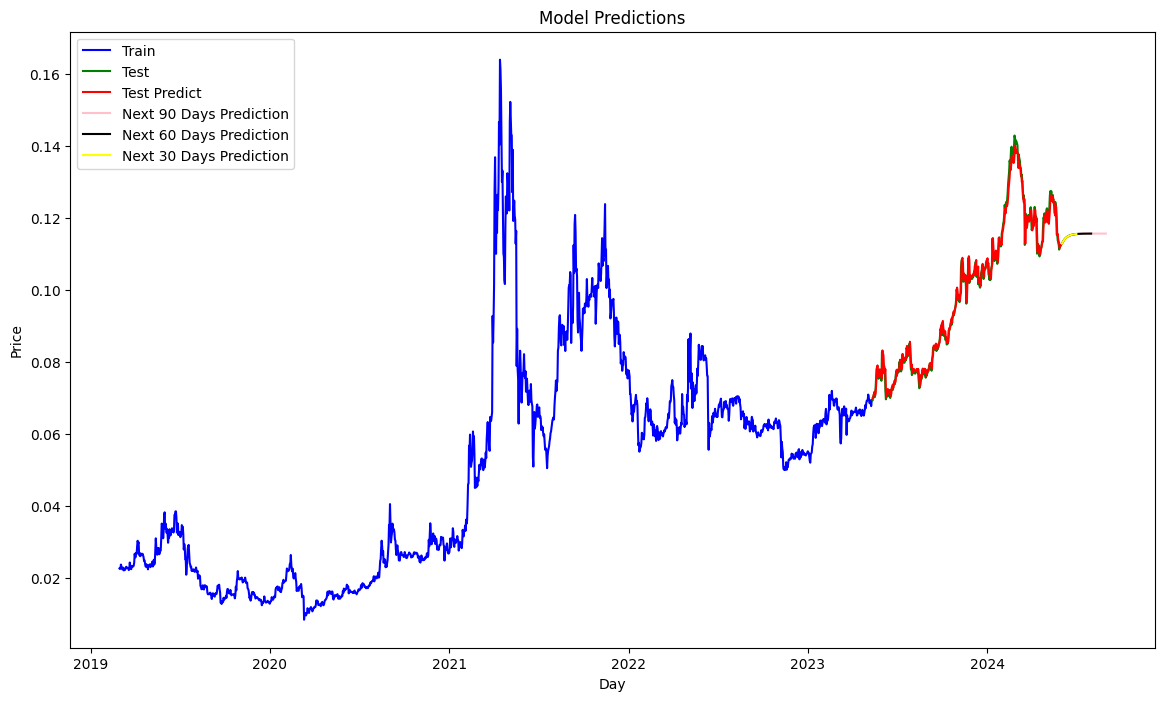
\includegraphics[width=\linewidth]{Image/MLP/MLP_TRON_82_new.png}
    \caption{MLP model's result with 8:2 splitting proportion}
    \label{fig:14}
  \end{minipage}
\end{figure}
\vspace{-2mm}
\subsection{BNB dataset}
\vspace{-2mm}
\begin{table}[H]
  \centering
  \begin{tabular}{|c|c|c|c|c|}
    \hline
    \multicolumn{5}{|c|}{\textbf{BNB Dataset's Evaluation}}                                             \\
    \hline
    \centering Model       & Training:Testing & RMSE             & MAPE (\%)       & MSE                \\
    \hline
    \multirow{2}{*}{LR}    & 7:3              & 250.279          & 86.40           & 62639.603          \\ & 8:2 &  196.348 & 69.72 & 38552.750 \\ & \textbf{9:1}&\textbf{131.961}&\textbf{32.73}&\textbf{17413.947}\\
    \hline
    \multirow{3}{*}{RNN}   & 7:3              & 20.28            & 5.19            & 411.22             \\
                           & \textbf{8:2}     & \textbf{12.02}   & \textbf{1.9}    & \textbf{144.498}   \\
                           & 9:1              & 16.68            & 2.95            & 278.129            \\
    \hline
    \multirow{2}{*}{GRU}   & \textbf{7:3}     & \textbf{13.270}  & \textbf{2.160}  & \textbf{176.090}   \\ &  8:2& 14.592 &2.425&	212.925 \\ & 9:1 & 15.475 & 2.175 & 239.472\\
    \hline
    \multirow{2}{*}{ARIMA} & \textbf{7:3}     & \textbf{116.788} & \textbf{26.463} & \textbf{13639.48}  \\ & 8:2 & 141.783 & 30.427 & 20102.409 \\ & 9:1 & 242.385 & 38.723 & 58750.813\\
    \hline
    \multirow{2}{*}{GARCH} & \textbf{7:3}     & \textbf{116.42}  & \textbf{26.75}  & \textbf{13553.28}  \\
                           & 8:2              & 141.23           & 30.42           & 19944.69           \\
                           & 9:1              & 239.61           & 38.07           & 57411.59           \\
    \hline
    \multirow{2}{*}{SES}   & \textbf{7:3}     & \textbf{116.764} & \textbf{26.36}  & \textbf{13633.898} \\ & 8:2 & 141.8623 & 30.32 & 20124.9178 \\ & 9:1 &  240.6164 &	38.27 & 57896.2456 \\
    \hline
    \multirow{2}{*}{LSTM}  & \textbf{7:3}     & \textbf{13.473}  & \textbf{2.38}   & \textbf{181.539}   \\ & 8:2 & 16.371 & 2.91 &  268.015 \\ & 9:1 & 17.907 &	2.40 & 320.663\\
    \hline
    \multirow{2}{*}{MLP}   & \textbf{7:3}     & \textbf{10.894}  & \textbf{0.020}  & \textbf{118.682}   \\ & 8:2 & 11.968 & 0.020 &  143.245 \\ & 9:1 & 15.366 & 0.022 & 236.119\\
    \hline
  \end{tabular}
  \caption{BNB Dataset's Evaluation}
  \label{mbbresult}
\end{table}
\vspace{-10mm}
\begin{figure}[H]
  \centering
  \begin{minipage}{0.8\linewidth}
    \centering
    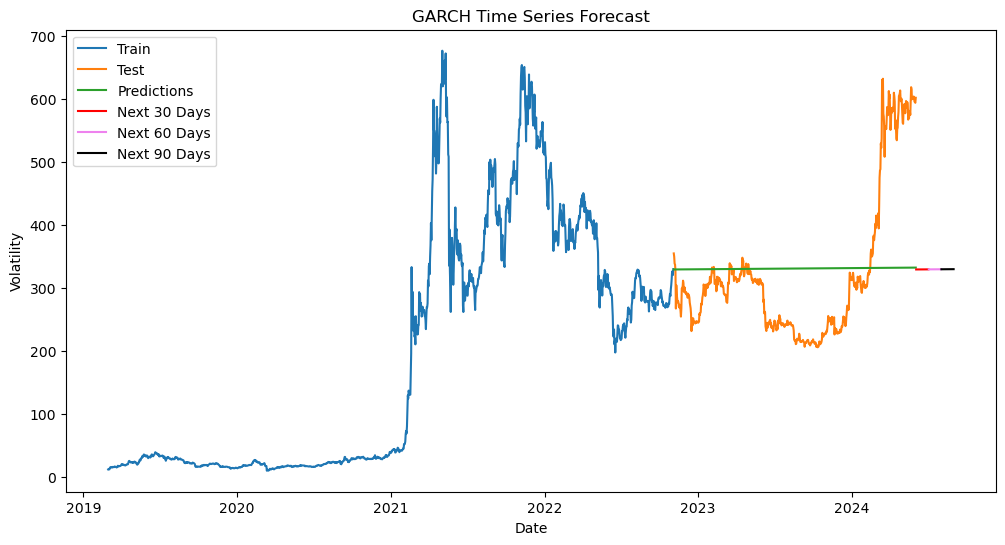
\includegraphics[width=\linewidth]{Image/Garch/GARCH_BNB73.png}
    \caption{GARCH model's result with 7:3 splitting proportion}
    \label{fig:15}
  \end{minipage}
\end{figure}
\vspace{-5mm}
\begin{figure}[H]
  \centering
  \begin{minipage}{0.8\linewidth}
    \centering
    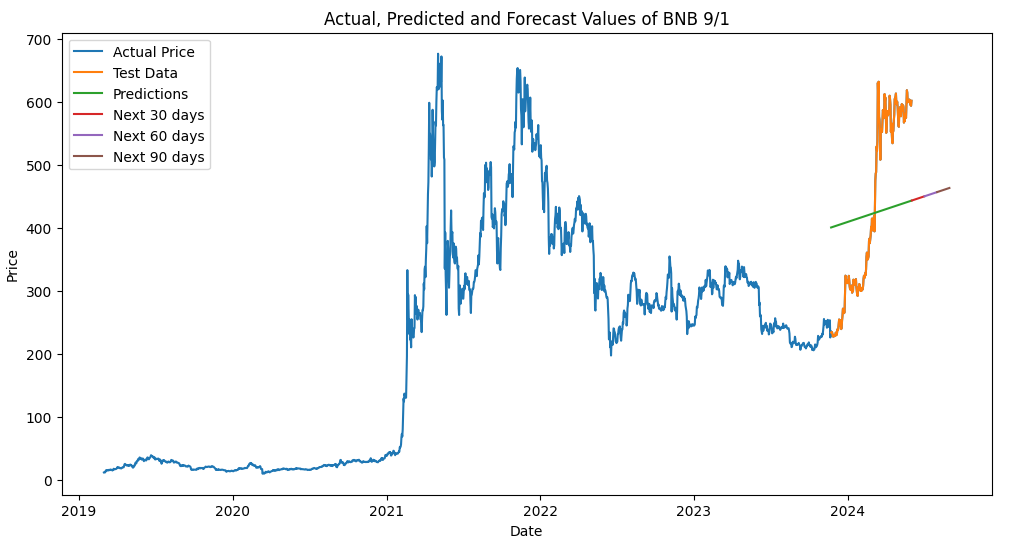
\includegraphics[width=\linewidth]{Image/LN/LN_BNB_91.png}
    \caption{LR model's result with 9:1 splitting proportion}
    \label{fig:16}
  \end{minipage}
\end{figure}
\vspace{-5mm}
\begin{figure}[H]
  \centering
  \begin{minipage}{0.8\linewidth}
    \centering
    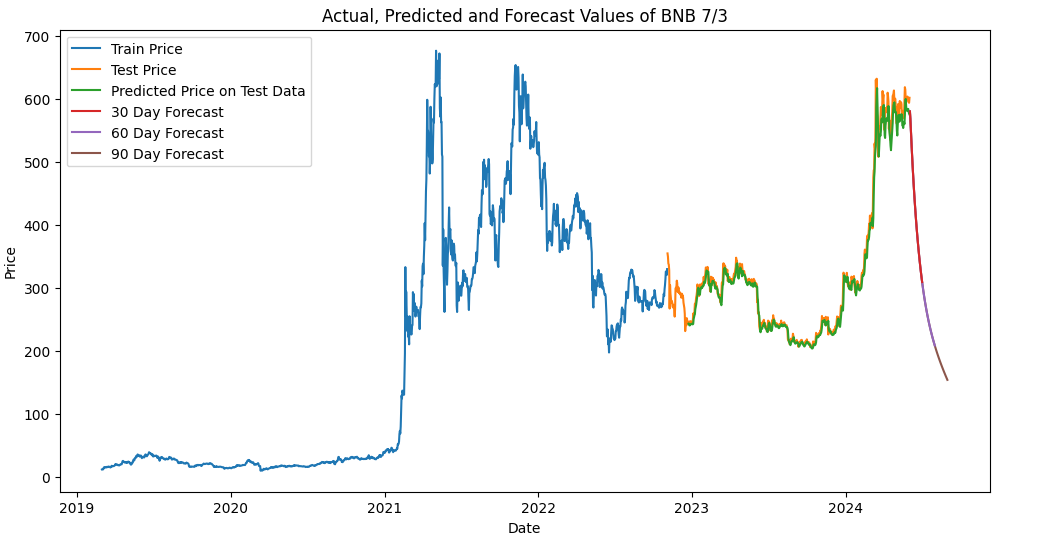
\includegraphics[width=\linewidth]{Image/LSTM/LSTM_BNB_73.png}
    \caption{LSTM model's result with 7:3 splitting proportion}
    \label{fig:17}
  \end{minipage}
\end{figure}
\vspace{-5mm}
\begin{figure}[H]
  \centering
  \begin{minipage}{0.8\linewidth}
    \centering
    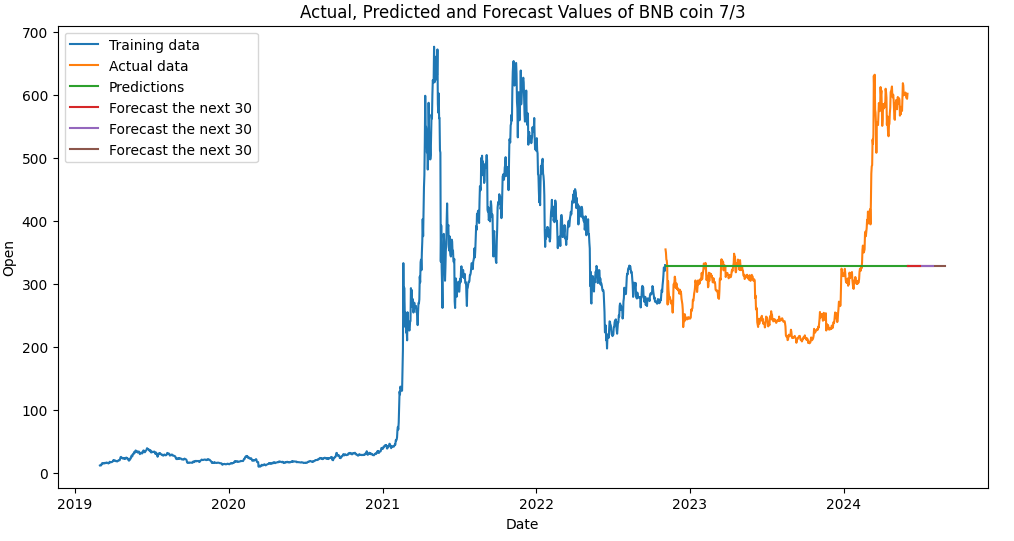
\includegraphics[width=\linewidth]{Image/SES/SES_BNB_73.png}
    \caption{SES model's result with 7:3 splitting proportion}
    \label{fig:18}
  \end{minipage}
\end{figure}
\vspace{-5mm}
\begin{figure}[H]
  \centering
  \begin{minipage}{0.8\linewidth}
    \centering
    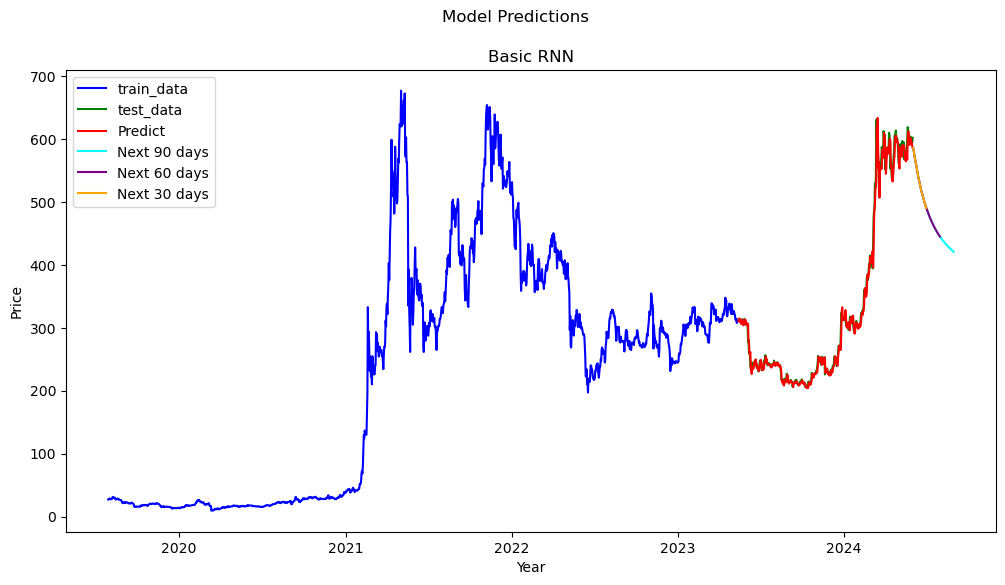
\includegraphics[width=\linewidth]{Image/RNN/RNN_BNB82.png}
    \caption{RNN model's result with 8:2 splitting proportion}
    \label{fig:19}
  \end{minipage}
\end{figure}
\vspace{-5mm}
\begin{figure}[H]
  \centering
  \begin{minipage}{0.8\linewidth}
    \centering
    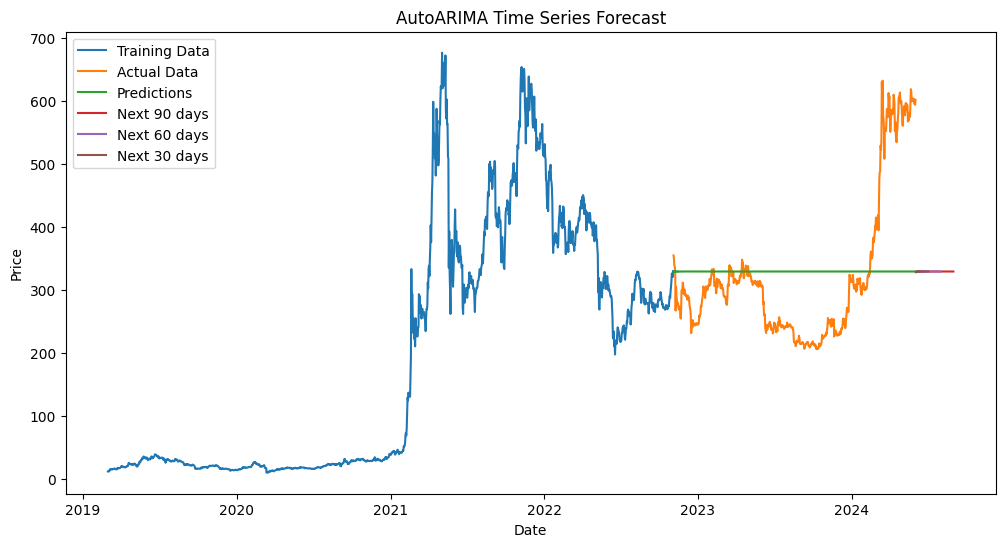
\includegraphics[width=\linewidth]{Image/Arima/Arima_BNB_7_3_n.png}
    \caption{ARIMA model's result with 7:3 splitting proportion}
    \label{fig:20}
  \end{minipage}
\end{figure}
\vspace{-5mm}
\begin{figure}[H]
  \centering
  \begin{minipage}{0.8\linewidth}
    \centering
    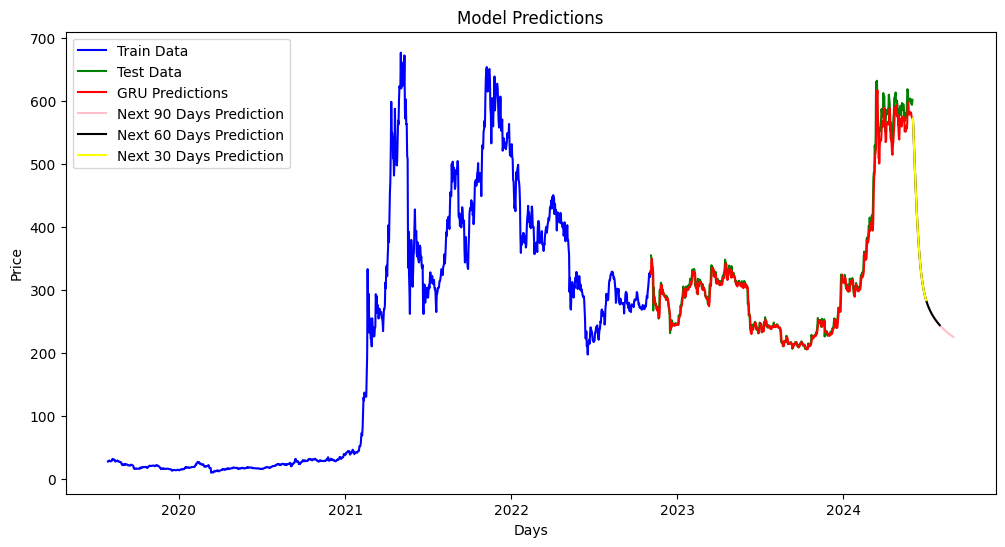
\includegraphics[width=\linewidth]{Image/GRU/GRU_BNN_73_n.png}
    \caption{GRU model's result with 7:3 splitting proportion}
    \label{fig:21}
  \end{minipage}
\end{figure}
\vspace{-10mm}
\begin{figure}[H]
  \centering
  \begin{minipage}{0.8\linewidth}
    \centering
    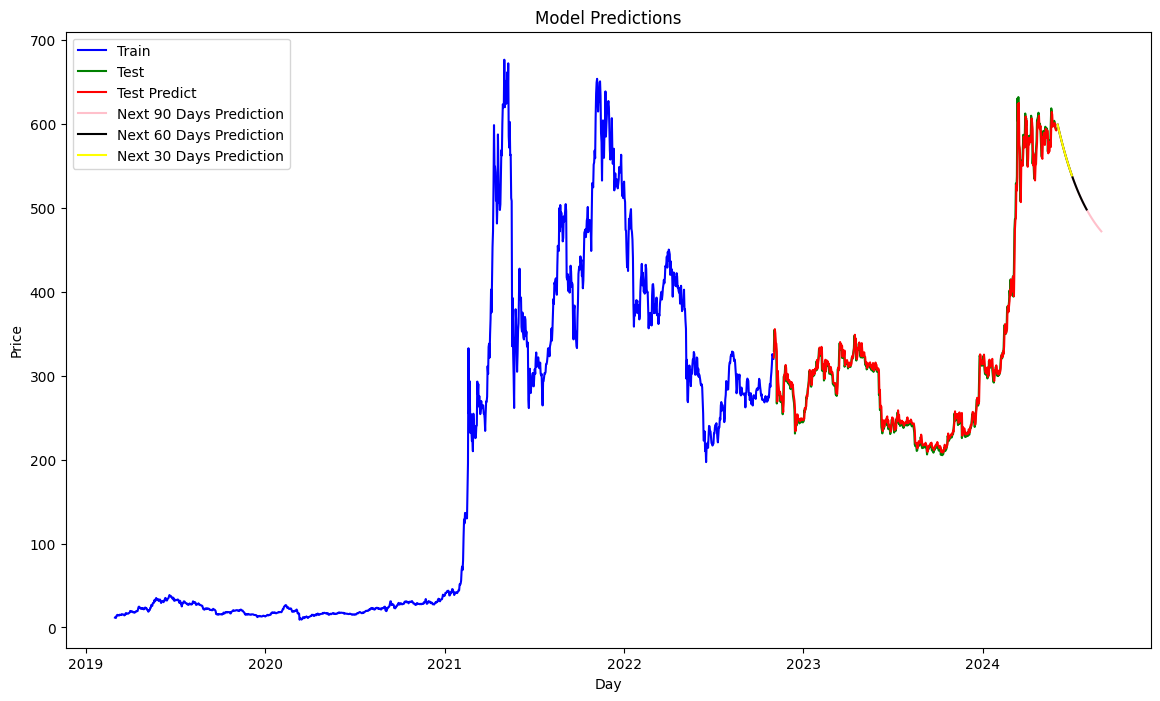
\includegraphics[width=\linewidth]{Image/MLP/MLP_BNB_7_3_new.png}
    \caption{MLP model's result with 7:3 splitting proportion}
    \label{fig:22}
  \end{minipage}
\end{figure}
\vspace{-3mm}
\subsection{Dogecoin dataset}
\vspace{-6mm}
\begin{table}[H]
  \centering
  \begin{tabular}{|c|c|c|c|c|}
    \hline
    \multicolumn{5}{|c|}{\textbf{DOGECOIN Coin Dataset's Evaluation}}                                \\
    \hline
    \centering Model       & Training:Testing & RMSE            & MAPE (\%)      & MSE               \\
    \hline
    \multirow{2}{*}{LR}    & 7:3              & 0.1336          & 163.61         & 0.0179            \\ & 8:2 &  0.0872 & 108.02 & 0.0076 \\ & \textbf{9:1} & \textbf{0.0428} & \textbf{37.72} & \textbf{0.0018} \\
    \hline
    \multirow{3}{*}{RNN}   & 7:3              & 0.008           & 7.37           & 5.82              \\ & \textbf{8:2} & \textbf{0.0096} & \textbf{9.547} & \textbf{9.144} \\ & 9:1 & 0.01 & 7.07 & 0.0001 \\
    \hline
    \multirow{2}{*}{GRU}   & 7:3              & 0.006           & 4.060          & 0.000033          \\ &  \textbf{8:2} & \textbf{0.006} &  \textbf{3.083} & \textbf{0.000035} \\ & 9:1 & 0.008 & 3.777 & 0.000064\\
    \hline
    \multirow{2}{*}{ARIMA} & 7:3              & 0.0198          & 17.739         & 0.0003            \\ & 8:2 & 0.013 &15.159 & 0.0001 \\ & \textbf{9:1} & \textbf{0.008} & \textbf{3.881} & \textbf{0.000069}\\
    \hline
    \multirow{3}{*}{GARCH} & 7:3              & 0.05            & 66.25          & 0.003             \\
                           & 8:2              & 0.047           & 56.21          & 0.002             \\
                           & \textbf{9:1}     & \textbf{0.037}  & \textbf{25.25} & \textbf{0.001}    \\
    \hline
    \multirow{2}{*}{SES}   & 7:3              & 0.0469          & 56.26          & 0.0022            \\ & \textbf{8:2} & \textbf{0.0471} & \textbf{22.39} & \textbf{0.0022} \\ & 9:1 &  0.0635 & 32.07 & 0.0040 \\
    \hline
    \multirow{2}{*}{LSTM}  & \textbf{7:3}     & \textbf{0.0064} & \textbf{4.32}  & \textbf{0.000040} \\ & 8:2 & 0.0071 & 4.47 &  0.000051 \\ & 9:1&  0.0099 &4.88 & 0.000098\\
    \hline
    \multirow{2}{*}{MLP}   & \textbf{7:3}     & \textbf{0.005}  & \textbf{0.031} & \textbf{0.000028} \\ & 8:2 & 0.006 &  0.037 &  0.000037 \\ & 9:1 & 0.009 & 0.057 & 0.000088\\
    \hline
  \end{tabular}
  \caption{DogeCoin Dataset's Evaluation}
  \label{dogecoinresult}
\end{table}
\vspace{-5mm}
\begin{figure}[H]
  \centering
  \begin{minipage}{0.8\linewidth}
    \centering
    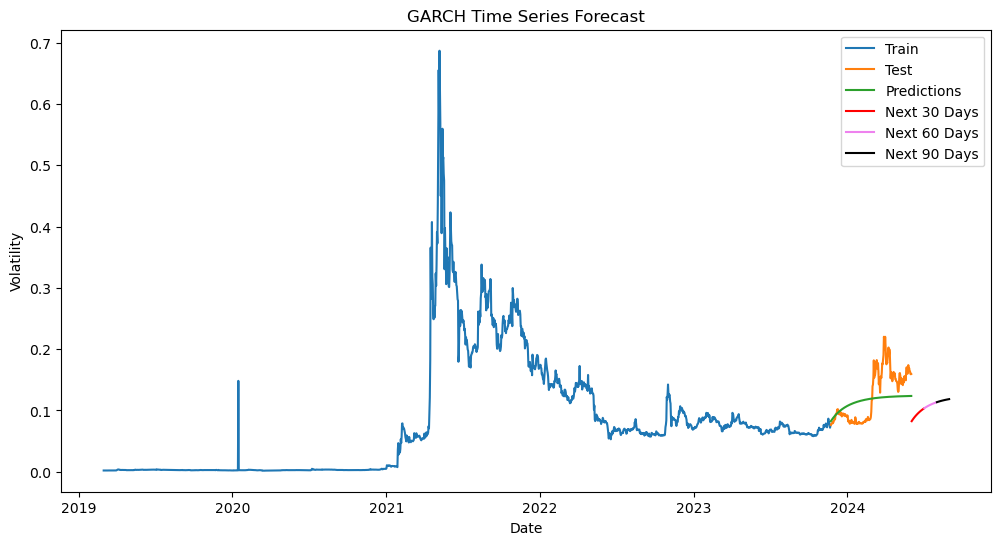
\includegraphics[width=\linewidth]{Image/Garch/GARCH_Dogecoin91.png}
    \caption{GARCH model's result with 9:1 splitting proportion}
    \label{fig:23}
  \end{minipage}
\end{figure}
\vspace{-5mm}
\begin{figure}[H]
  \centering
  \begin{minipage}{0.8\linewidth}
    \centering
    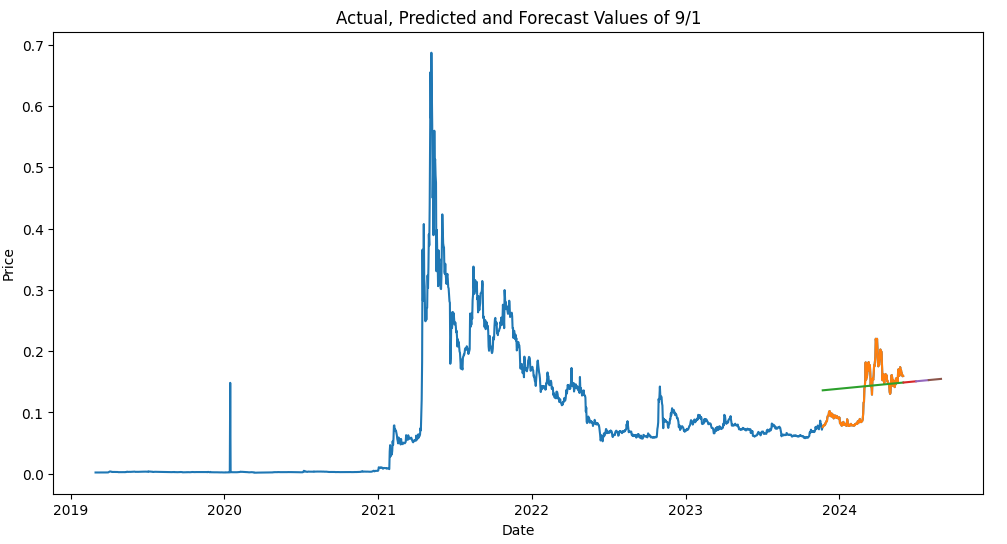
\includegraphics[width=\linewidth]{Image/LN/LN_DOGE_91.png}
    \caption{LR model's result with 9:1 splitting proportion}
    \label{fig:24}
  \end{minipage}
\end{figure}
\vspace{-5mm}
\begin{figure}[H]
  \centering
  \begin{minipage}{0.8\linewidth}
    \centering
    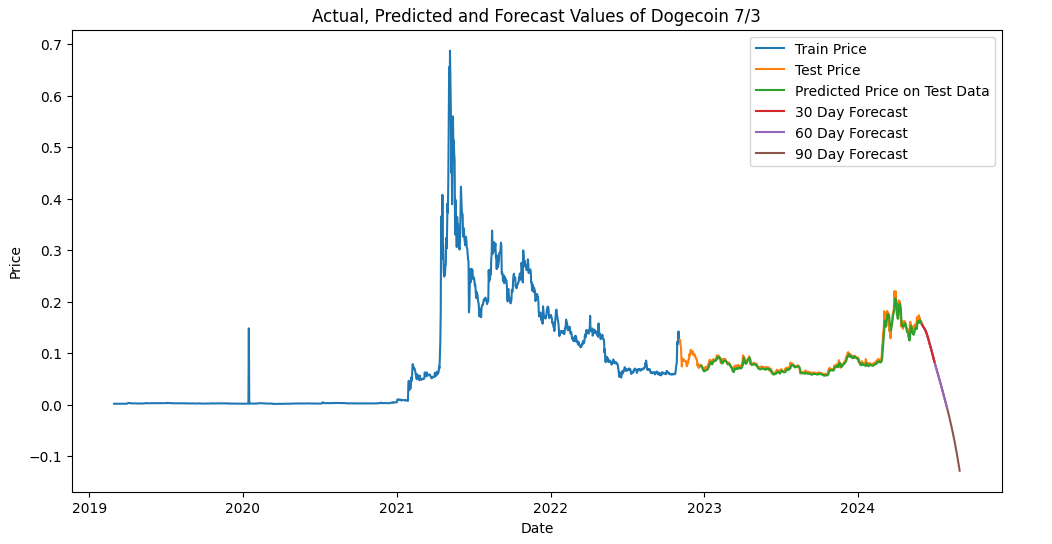
\includegraphics[width=\linewidth]{Image/LSTM/LSTM_DOGE_73.png}
    \caption{LSTM model's result with 7:3 splitting proportion}
    \label{fig:25}
  \end{minipage}
\end{figure}
\vspace{-5mm}
\begin{figure}[H]
  \centering
  \begin{minipage}{0.8\linewidth}
    \centering
    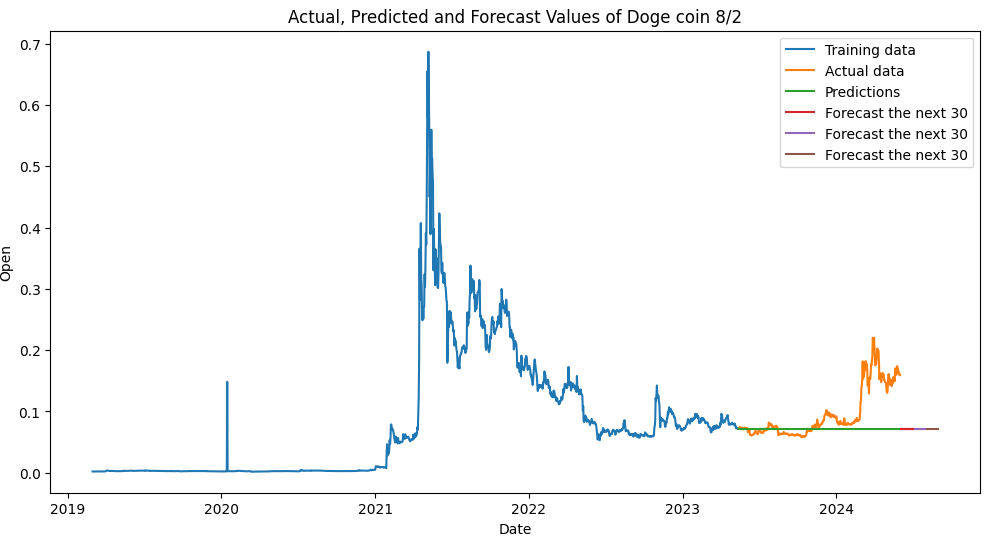
\includegraphics[width=\linewidth]{Image/SES/SES_DOGE_82.png}
    \caption{SES model's result with 8:2 splitting proportion}
    \label{fig:26}
  \end{minipage}
\end{figure}
\vspace{-5mm}
\begin{figure}[H]
  \centering
  \begin{minipage}{0.8\linewidth}
    \centering
    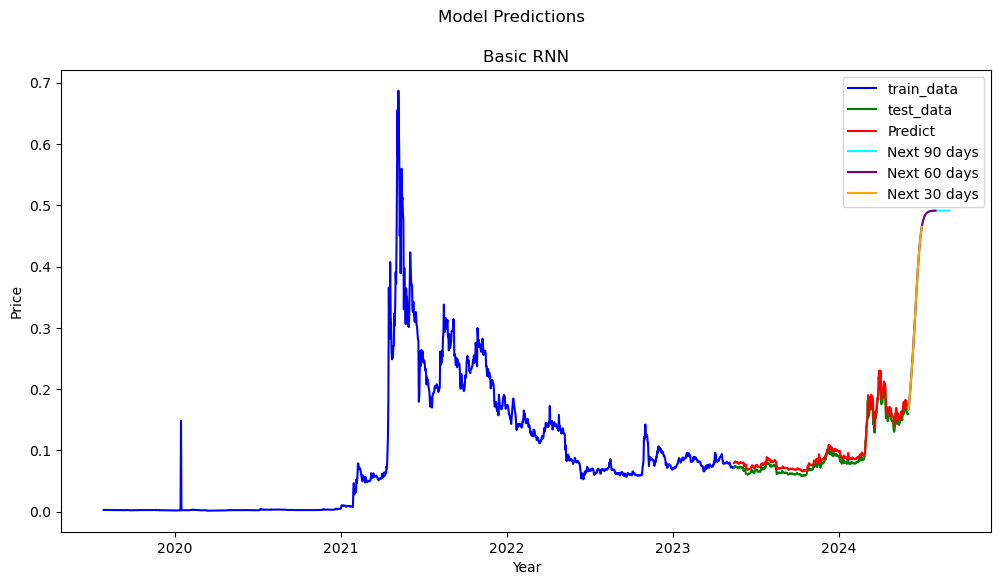
\includegraphics[width=\linewidth]{Image/RNN/RNN_Dogecoin82.png}
    \caption{RNN model's result with 8:2 splitting proportion}
    \label{fig:27}
  \end{minipage}
\end{figure}
\vspace{-5mm}
\begin{figure}[H]
  \centering
  \begin{minipage}{0.8\linewidth}
    \centering
    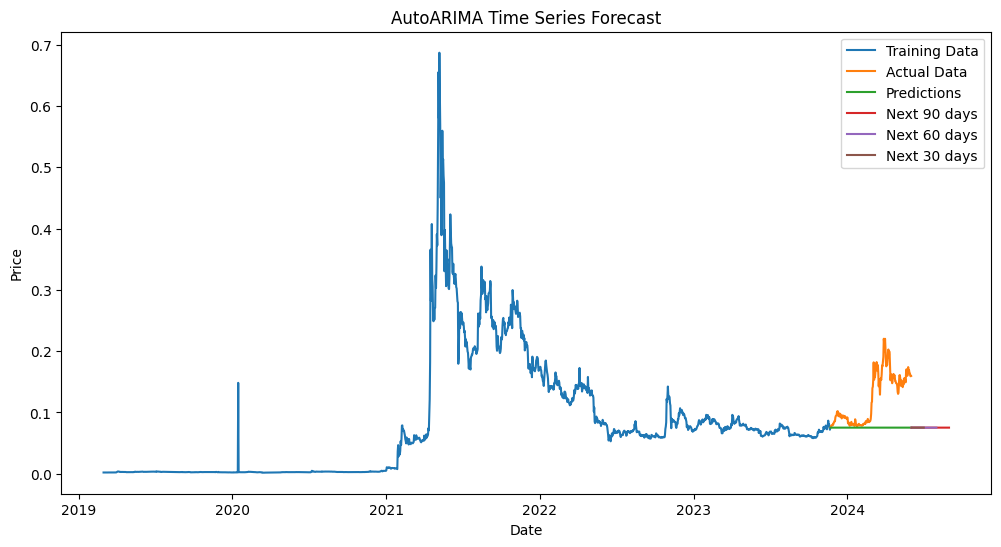
\includegraphics[width=\linewidth]{Image/Arima/Arima_doge_9_1_n.png}
    \caption{ARIMA model's result with 9:1 splitting proportion}
    \label{fig:28}
  \end{minipage}
\end{figure}
\vspace{-5mm}
\begin{figure}[H]
  \centering
  \begin{minipage}{0.8\linewidth}
    \centering
    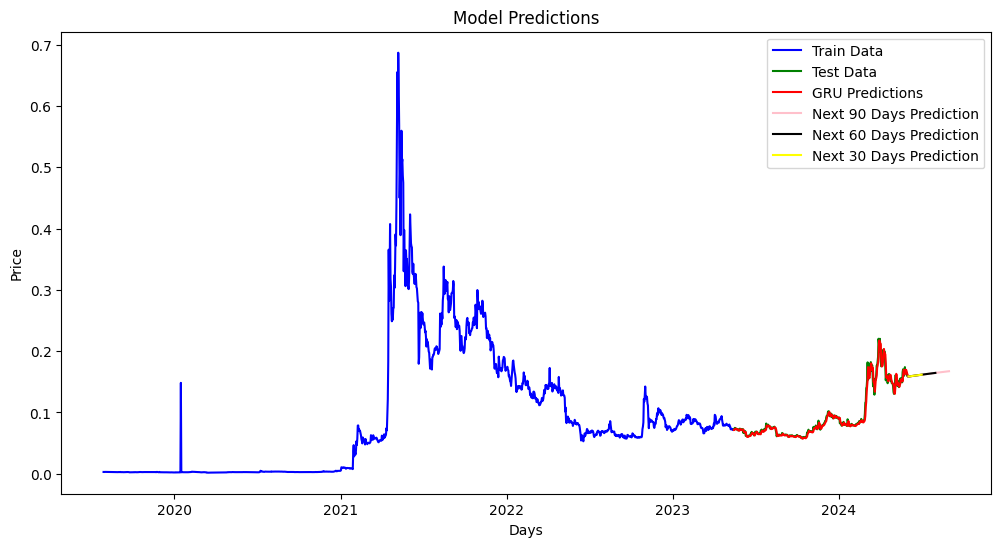
\includegraphics[width=\linewidth]{Image/GRU/GRU_DOGE_82_n.png}
    \caption{GRU model's result with 8:2 splitting proportion}
    \label{fig:29}
  \end{minipage}
\end{figure}
\vspace{-5mm}
\begin{figure}[H]
  \centering
  \begin{minipage}{0.8\linewidth}
    \centering
    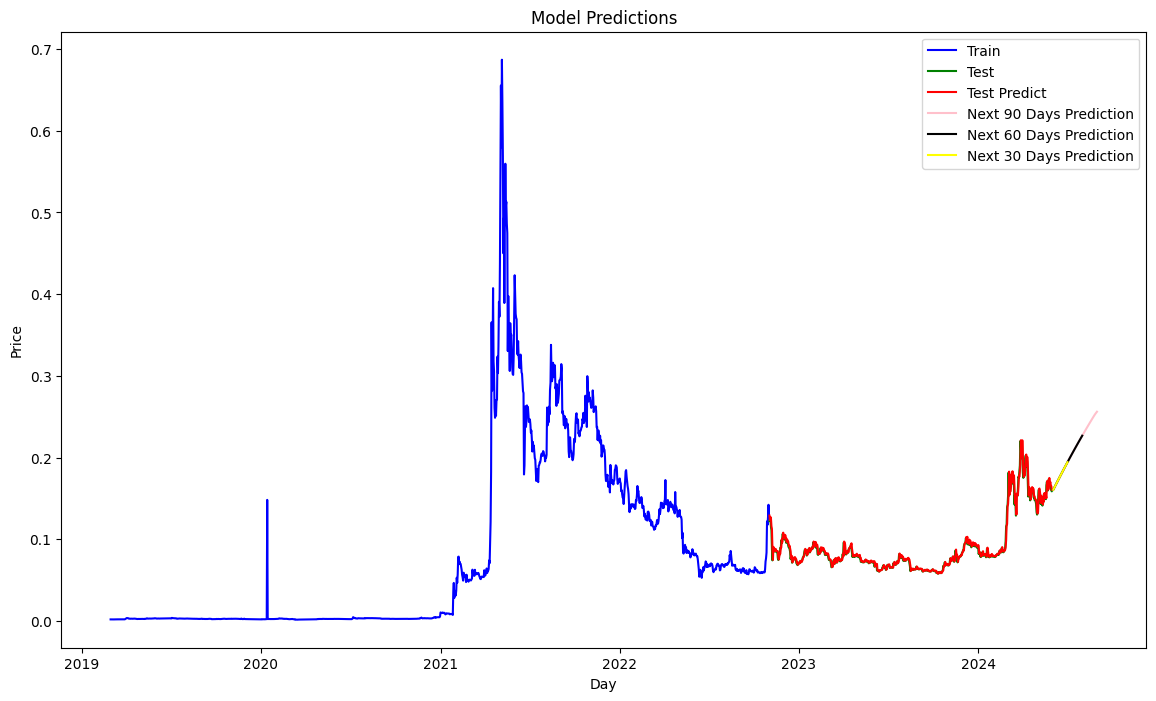
\includegraphics[width=\linewidth]{Image/MLP/MLP_DOGE_73_new.png}
    \caption{MLP model's result with 7:3 splitting proportion}
    \label{fig:30}
  \end{minipage}
\end{figure}
\section{Conclusion}
\subsection{Summary}
In the pursuit of predicting cryptocurrency prices, various methodologies have been explored, spanning from conventional statistical models to sophisticated machine learning algorithms. Among these, MLP (Multi-Layer Perceptron) and GRU (Gated Recurrent Unit) algorithms generally outperform other methods such as SES (Simple Exponential Smoothing), Linear Regression, RNN (Recurrent Neural Network), ARIMA (AutoRegressive Integrated Moving Average), LSTM (Long Short-Term Memory) and GARCH (Generalized Autoregressive Conditional Heteroskedasticity). MLP and GRU are highly effective due to their capability to understand and adapt to intricate temporal patterns in time-series data. They excel in handling non-linear trends, long-term relationships, and erratic fluctuations commonly seen in cryptocurrency markets. LSTM networks are particularly adept at retaining information across extended sequences, which is crucial for modeling price trends that evolve over time amid varying levels of market volatility. \\
In contrast, simpler methods like SES and Linear Regression may struggle with the inherent complexities and nonlinearities inherent in cryptocurrency price data. While RNNs offer more flexibility, they can encounter challenges such as gradient vanishing and difficulty in learning dependencies over extended periods. ARIMA models are suitable for stationary series but may not adequately capture the dynamic and irregular patterns of cryptocurrency prices. MLPs are robust in learning complex relationships but may require extensive tuning and regularization for effective performance on time-series data. GARCH models are suitable for volatility modeling but do not directly forecast price levels.\\
In conclusion, GRU and MLP models stand out in cryptocurrency price prediction due to their ability to handle complex data patterns and effectively capture long-term dependencies. These models demonstrate their suitability for achieving accurate and reliable forecasts in the specialized domain of cryptocurrency price prediction.
\vspace{-2mm}
\subsection{Future Considerations}
In our future research endeavors, it is paramount to prioritize further refining the models previously discussed. This optimization initiative should focus on several key areas
\indent\textbullet\ Focus on interpretability and explainability, as models grow in complexity, ensuring they remain interpretable is crucial for stakeholders to trust and act upon forecasting insights. Techniques such as model explainability tools and transparent methodologies should be integrated to enhance trustworthiness and usability.\\
\indent\textbullet\ Enhancing model accuracy , while the aforementioned algorithms have shown promise in predicting cryptocurrency prices, there remains a pressing need to elevate their accuracy for more precise forecasting outcomes. This involves not only improving existing algorithms but also exploring advanced techniques such as feature engineering and hyperparameter tuning to maximize predictive performance.\\
\indent\textbullet\ Innovating new forecasting models, the landscape of forecasting is continuously evolving, necessitating ongoing exploration of cutting-edge models and methodologies. This includes researching novel forecasting techniques that integrate alternative data sources (e.g., sentiment analysis from social media or macroeconomic indicators) to capture nuanced market behaviors more effectively. \\
By continually exploring new avenues for improvement, integrating cutting-edge technologies, and expanding the scope of data inputs, we aim to continuously optimize forecasting models. This proactive approach not only enhances their precision and reliability in predicting cryptocurrency prices but also equips us to navigate the dynamic landscape of financial markets with greater confidence and foresight.
\section*{Acknowledgment}
\addcontentsline{toc}{section}{Acknowledgment}
Above all, we deeply appreciate the guidance and expertise provided by \textbf{Assoc. Prof. Dr. Nguyen Dinh Thuan} and \textbf{Mr. Nguyen Minh Nhut} throughout our research journey. Their mentorship and invaluable feedback have played a pivotal role in shaping the direction and quality of this study. Their extensive knowledge, critical insights, and meticulous attention to detail have significantly contributed to the achievements of this research.
\\We are sincerely grateful to our mentors for their unwavering support and contributions, without which this research would not have been possible. We extend heartfelt thanks to everyone involved for their invaluable assistance, encouragement, and belief in our work.

%% UNCOMMENT these lines below (and remove the 2 commands above) if you want to embed the bibliografy.
\begin{thebibliography}{00}
  \bibitem{b1} Bollerslev, T. (1986). Generalized autoregressive conditional heteroskedasticity. Journal of Econometrics, 31(3), 307-327.
  \bibitem{b2} Brown, R. G. (1956). Exponential smoothing for predicting demand. Management Science, 6(3), 324-342.
  \bibitem{b3} Ben Abdallah, M., Fekete Farkas, M., \& Lakner, Z. (2020). Analysis of meat price volatility and volatility spillovers in Finland. Agricultural Economics, 66, 84–91.
  \bibitem{b4} Saleem, A., Bárczi, J., \& Sági, J. (2021). COVID-19 and Islamic Stock Index: Evidence of Market Behavior and Volatility Persistence. Journal of Risk and Financial Management, 14, 389.
  \bibitem{b5} Hansen, P. R., \& Lund, T. (2004). A Forecast Comparison of Volatility Models: Does Anything Beat a GARCH(1,1)?. Journal of Applied Econometrics, 20(7), 873-889.
  \bibitem{b6} Kim, J.-M., Kim, D. H., \& Jung, H. (2021). Estimating yield spreads volatility using GARCH-type models. The North American Journal of Economics and Finance, 57, 101396.
  \bibitem{b7} Zhang, H., et al. (2019). Multilayer Perceptron Models for Bitcoin Price Forecasting. Neural Computing and Applications, 32(7), 1987-2000.
  \bibitem{b8} Box, G. E. P., Jenkins, G. M., Reinsel, G. C., \& Ljung, G. M. (2015). Time Series Analysis: Forecasting and Control (5th ed.). John Wiley \& Sons.
  \bibitem{b9} Hyndman, R. J., \& Athanasopoulos, G. (2018). Forecasting: Principles and Practice (2nd ed.). OTexts.
  \bibitem{b10} Kumar, R., \& Thenmozhi, M. (2006). Predicting Stock Prices Using Linear Regression. [Details missing].
  \bibitem{b11} Zhang, Y., Zhang, G., \& Zhang, J. (2019). Forecasting Bitcoin Prices Using RNN.
  \bibitem{b12} Chung, J., Gulcehre, C., Cho, K., \& Bengio, Y. (2014). Empirical Evaluation of Gated Recurrent Neural Networks on Sequence Modeling. arXiv preprint arXiv:1412.3555.
  \bibitem{b13} Tsai, C.-F., Lin, Y.-C., Yen, D. C., \& Chen, Y.-M. (2010). Predicting Stock Prices Using Hybrid ARIMA and Genetic Algorithms.
  \bibitem{b14} Aras, S. (2021). Stacking hybrid GARCH models for forecasting Bitcoin volatility. Expert Systems with Applications, 174, 114747.
  \bibitem{b15} Fischer, T., \& Krauss, C. (2018). Deep Learning with Long Short-Term Memory Networks for Financial Market Predictions.
  \bibitem{b16} Goodfellow, I., Bengio, Y., \& Courville, A. (2016). Deep Learning. MIT Press.
  \bibitem{b17} Lipton, Z. C., Berkowitz, J., \& Elkan, C. (2015). A Critical Review of Recurrent Neural Networks for Sequence Learning. arXiv preprint arXiv:1506.00019.
  \bibitem{b18} Graves, A. (2012). Supervised Sequence Labelling with Recurrent Neural Networks. Studies in Computational Intelligence, 385, Springer.
  \bibitem{b19} Cryer, J. D., \& Chan, K. S. (2008). Time series analysis: with applications in R. Springer Science \& Business Media.
  \bibitem{b20} Cho, K., et al. (2014). Learning Phrase Representations using RNN Encoder-Decoder for Statistical Machine Translation. arXiv preprint arXiv:1406.1078.
  \bibitem{b21} Bibi, I., Akhunzada, A., Malik, J., Iqbal, J., Musaddiq, A., \& Kim, S. (2020). A Dynamic DL-Driven Architecture to Combat Sophisticated Android Malware. IEEE Access, PP. 1-1. 10.1109/ACCESS.2020.3009819.
  \bibitem{b22} Rumelhart, D. E., Hinton, G. E., \& Williams, R. J. (1986). Learning representations by back-propagating errors. Nature, 323(6088), 533-536.
  \bibitem{b23} Pan, H., Ye, Z., He, Q., Yan, C., Yuan, J., Lai, X., Su, J., \& Li, R. (2022). Discrete Missing Data Imputation Using Multilayer Perceptron and Momentum Gradient Descent. Sensors, 22, 5645. 10.3390/s22155645.
  \bibitem{b24} Hochreiter, S., \& Schmidhuber, J. (1997). Long Short-Term Memory. Neural Computation, 9(8), 1735-1780.
  \bibitem{b25} Olah, C. (2015). Understanding LSTM Networks. Retrieved from http://colah.github.io/posts/2015-08-Understanding-LSTMs/.
  \bibitem{b26} Hyndman, R. J., \& Athanasopoulos, G. (n.d.). 7.1 Simple Exponential Smoothing. In Forecasting: Principles and Practice (2nd ed.). Retrieved from https://otexts.com/fpp2/simple-smoothing.html.
  \bibitem{b27} Hyndman, R. J., \& Athanasopoulos, G. (n.d.). Chapter 8 Exponential Smoothing. In Forecasting: Principles and Practice (3rd ed.). Retrieved from https://otexts.com/fpp3/expsmooth.html.
  \bibitem{b28} Frost, J. (n.d.). Linear regression. Statistics By Jim. Retrieved from https://statisticsbyjim.com/regression/linear-regression/.
  \bibitem{b29} Taylor, S. (2023). Regression analysis. Corporate Finance Institute. Retrieved from https://corporatefinanceinstitute.com/resources/data-science/regression-analysis/.
  \bibitem{b30} Ostertagova, Eva \& Ostertag, Oskar. (2011). The Simple Exponential Smoothing Model. 
\end{thebibliography}

%%%%%%%%%%%%%%%


\EOD

\end{document}
